\documentclass{beamer}
\mode<presentation>
\usetheme{CambridgeUS}
\usepackage[russian]{babel}
\usepackage[utf8]{inputenc}
\usepackage[T2A]{fontenc}
\usepackage{sansmathaccent}

\usepackage{verbatim}
\usepackage{alltt}

\pdfmapfile{+sansmathaccent.map}
\title[Artifical Intelligence]{Деревья поиска}
\author{Наумов Д.А., доц. каф. КТ}
\date[05.11.2019] {Экспертные системы и искусственный интеллект, 2019}

\begin{document}

%ТИТУЛЬНЫЙ СЛАЙД
\begin{frame}
  \titlepage
\end{frame}
  
%СОДЕРЖАНИЕ ЛЕКЦИИ
\begin{frame}
  \frametitle{Содержание лекции}
  \tableofcontents  
\end{frame}

\begin{frame}{Деревья поиска}
Игры с единственным игроком подобны деревьям игр:
\begin{itemize}
\item имеется начальное состояние - верхний узел в дереве поиска;
\item имеется последовательность ходов, которая изменяет позицию на доске до тех пор, пока не будет достигнуто целевое состояние. 
\end{itemize} 
\begin{block}{Дерево поиска}
представляет набор промежуточных состояний доски в процессе выполнения
алгоритма поиска пути. 
\end{block}
\begin{block}{Структура данных для дерева поиска}
представляет собой дерево, так как алгоритм гарантирует, что он не посещает никакое состояние доски дважды. 
\end{block}
\begin{block}{Цель алгоритма}
определеить, в каком порядке следует посещать состояния доски в попытках достичь целевого состояния.
\end{block}
\end{frame}

\begin{frame}
\begin{minipage}{0.5\textwidth}
\begin{flushleft}
\begin{enumerate}
\item головоломка <<8>>, играется на доске 3x3, 
\item восемь квадратных плиток, пронумерованных от 1 до 8, и пустое пространство, в котором плитки нет. 
\item соседняя (по горизонтали или вертикали) клитка может быть перемещена путем сдвига в пустое пространство; 
\item цель: начав с начального состояния, перемещая плитки, достичь целевого состояния.
\end{enumerate}
\end{flushleft}
\end{minipage}
%\hfill
\begin{minipage}{0.3\textwidth}
\begin{flushright}
\begin{figure}[h]
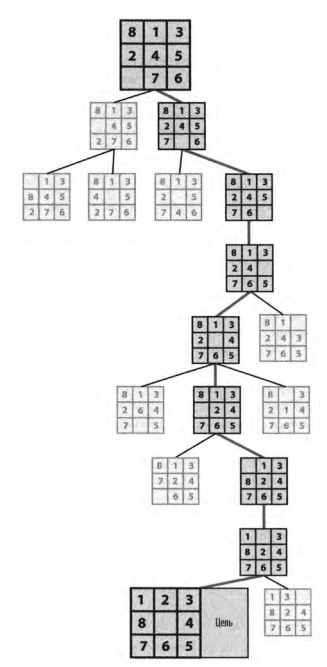
\includegraphics[scale=0.5]{images/lec06-pic01.png}
\end{figure}
\end{flushright}
\end{minipage}
\end{frame}

\begin{frame}{Алгоритмы поиска}
Слепой поисковый алгоритм использует фиксированную стратегию вместо вычисления состояния доски. 
\begin{block}{Слепой поиск в глубину}
просто играет в игру, произвольно выбирая очередной ход из доступных вариантов для данного состояния доски и выполняя откат при достижении максимальной глубины расширения.
\end{block}
\begin{block}{Слепой поиск в ширину}
методично исследует все возможные решения с $k$ ходами перед тем
как испытать любое решение с $k+1$ ходами.
\end{block}
\begin{block}{Алгоритм A*Search}
выполняется поиск решения с использованием различных эвристических функций. 
\end{block}
\end{frame}

\begin{frame}{Эвристические функции}
\begin{block}{Эвристические функции }
оценивают количество оставшихся ходов до целевого состояния из данного и могут использоваться для непосредственного поиска пути. 
\end{block}
Например, в головоломке <<8>> такая функция будет оценивать для каждой плитки в состоянии доски число ходов, необходимых для ее размещения в нужном месте в целевом состоянии. 

Наибольшая трудность в поиске пути состоит в разработке эффективной эвристической функции. 
\end{frame}

\section{Поиск в глубину}
\begin{frame}{Поиск в глубину}
\textbf{Поиск в глубину} пытается найти путь к целевому состоянию доски, делая столько ходов вперед, сколько возможно. 
\begin{itemize}
\item некоторые деревья поиска содержат очень большое количество состояний доски, поиск в глубину оказывается практичным, только
если максимальная глубина поиска фиксируется заранее;
\item для того, чтобы избежать зацикливания, необходимо запоминать уже рассмотренные состояния;
\item состояния, которые еще не посещены, - \textbf{открытые состояния}, помещаются в стек;
\item множество посещенных состояний - закрытые состояния доски. 
\end{itemize}
Алгоритм возвращает \textbf{последовательность ходов}, которая представляет собой путь от начального состояния к целевому (или сообщает, что такое решение не найдено).
\end{frame}

\begin{frame}{Поиск в глубину}
\begin{enumerate}
\item На каждой итерации поиск в глубину снимает со стека непосещенное состояние доски и расширяет его путем вычисления множества последующих состояний доски с учетом доступных разрешенных ходов. 
\item Поиск прекращается, когда достигнуто целевое состояние доски. 
\item Любой преемник состояния доски, который уже имеется во множестве закрытых состояний, отбрасывается. 
\item Оставшиеся непосещенные состояния доски помещаются в стек открытых состояний, и поиск продолжается.
\end{enumerate}
\end{frame}

\begin{frame}
\begin{figure}[h]
\centering
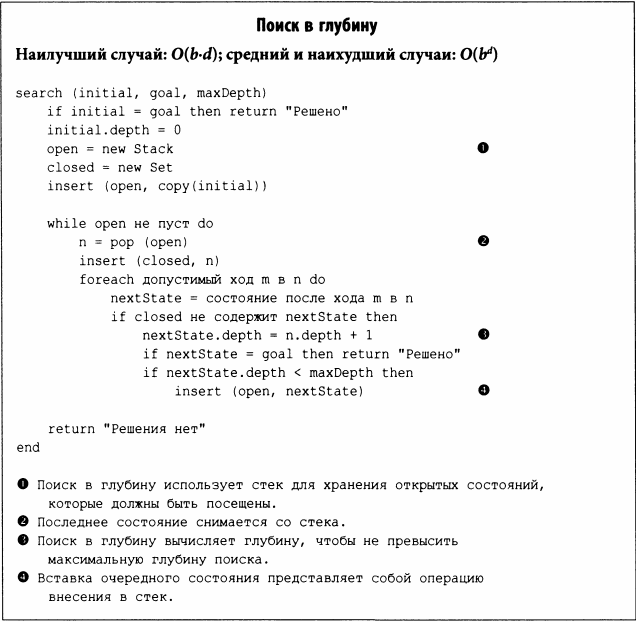
\includegraphics[scale=0.5]{images/lec06-pic02.png}
\end{figure}
\end{frame}

\begin{frame}
\begin{figure}[h]
\centering
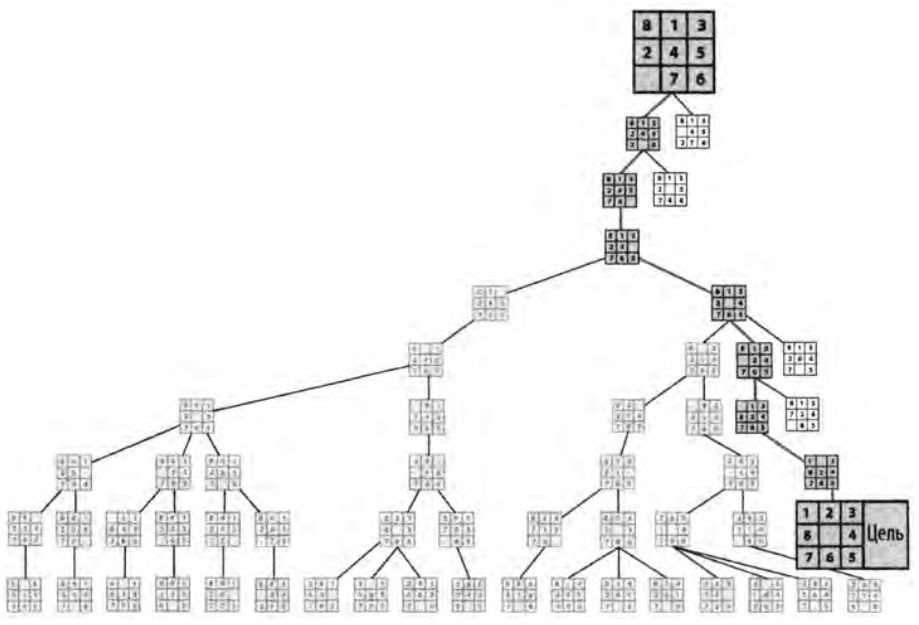
\includegraphics[scale=0.5]{images/lec06-pic03.png}
\end{figure}
\end{frame}

\begin{frame}{Анализ алгоритма поиска в глубину}
Пусть $d$ - максимальная глубина, ограничивающая поиск в глубину, а $b$ — коэффициент ветвления дерева поиска.

Производительность алгоритма определяется:
\begin{itemize}
\item общими характеристиками (базовые операции);
\item специфичными операции для конкретной задачи.
\end{itemize}

В общем случае замедлить работу алгоритма могут базовые операции:\begin{itemize}
\item Удаление очередного состояния доски для оценки.
\item Добавление состояния доски во множество закрытых состояний.
\item Определение наличия состояния во множестве закрытых состояний.
\item Добавление состояния доски во множество открытых состояний для позднейшего посещения.
\end{itemize}
\end{frame}

\begin{frame}{Анализ алгоритма поиска в глубину}
Специфическими для конкретной задачи характеристиками, которые влияют
на производительность, являются:
\begin{itemize}
\item количество состояний-преемников для отдельного состояния доски;
\item упорядочение допустимых ходов.
\end{itemize}
Если имеется какая-то эвристическая информация (какие ходы вероятнее других ведут к решению), то в упорядоченном списке допустимых ходов они должны появляться раньше прочих.
\begin{itemize}
\item В общем случае размер дерева поиска растет экспоненциально с основанием, равным коэффициенту ветвления $b$. 
\item У головоломки <<8>> коэффициент ветвления находится между 2 и 4, в зависимости от местоположения пустой плитки, и в среднем равен $2.67$. 
\end{itemize}
\end{frame}

\begin{frame}
Начальная позиция N2
\begin{figure}[h]
\centering
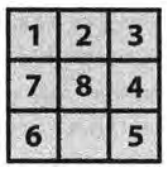
\includegraphics[scale=0.25]{images/lec06-pic04.png}
\end{figure}
Размер деревьев поиска для поиска в глубину с увеличением предельной глубины поиска:
\begin{figure}[h]
\centering
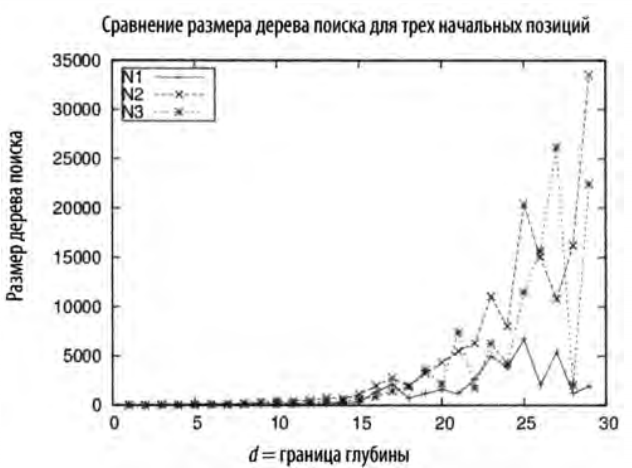
\includegraphics[scale=0.45]{images/lec06-pic05.png}
\end{figure}
\end{frame}

\section{Поиск в ширину}

\begin{frame}{Поиск в ширину}
\textbf{Поиск в ширину} пытается найти путь с помощью методичной оценки состояний доски, находящихся ближе всего к начальному состоянию.
\begin{itemize}
\item Кардинальным отличием от поиска в глубину является то, что поиск в ширину поддерживает очередь открытых и еще непосещенных состояний, в то время как поиск в глубину использует стек. 
\item На каждой итерации поиск в ширину удаляет из очереди очередное непосещенное состояние и расширяет его для вычисления множества состояний-преемников с учетом допустимых ходов. 
\item Если достигается целевое состояние, поиск прекращается. 
\item Любое состояние, имеющееся во множестве закрытых состояний, отбрасывается. Остальные непосещенные состояния добавляются в конец очереди открытых состояний, и поиск продолжается.
\end{itemize}
Поиск гарантированно находит кратчайший путь к целевому состоянию, если такой путь существует.
\end{frame}

\begin{frame}
\begin{figure}[h]
\centering
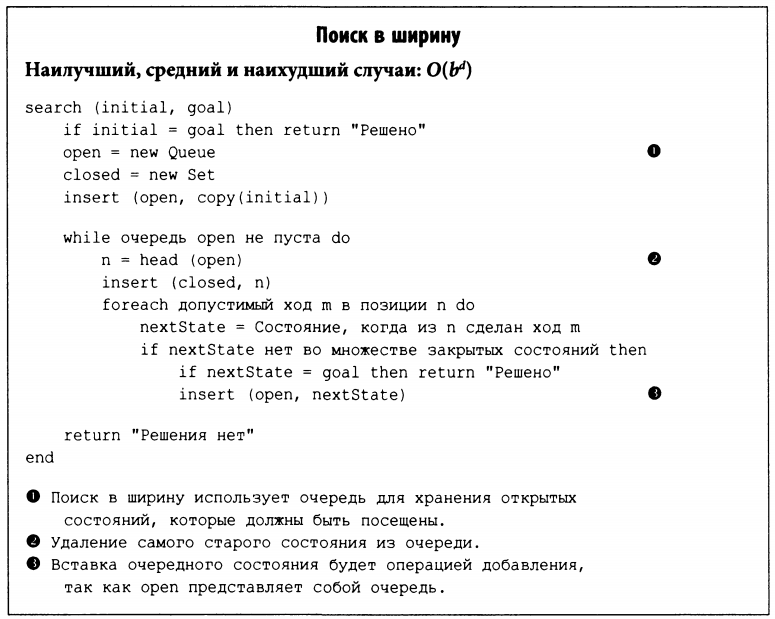
\includegraphics[scale=0.5]{images/lec06-pic07.png}
\end{figure}
\end{frame}

\begin{frame}{Анализ алгоритма поиска в ширину}
\begin{itemize}
\item Поиск должен хранить во множестве открытых состояний порядка $b^d$ состояний доски, где $b$ - коэффициент ветвления состояний
доски, a $d$ — глубина найденного решения (для поиска в глубину этот параметр равен $b\dot d$). 
\item Поиск в ширину гарантированно находит решение с наименьшим числом
ходов, которые преобразуют начальное состояние доски в целевое состояние.
\item Поиск добавляет состояние доски во множество открытых состояний, только если оно отсутствует во множестве закрытых состояний. 
\end{itemize}
\end{frame}

\section{A*Seacrh}

\begin{frame}{Алгоритм A*Search}
\begin{block}{A*Search}
представляет собой итеративный, упорядоченный поиск, который поддерживает набор открытых состояний доски, предназначенных для исследования в попытке достичь целевого состояния.
\end{block}
На каждой итерации \textit{A*Search} использует функцию оценки $f(n)$ для выбора того состояния доски $n$ из множества открытых состояний, для которого $f(n)$ имеет наименьшее значение.
\[f(n)=g(n)+h(n)\]
где
\begin{itemize}
\item $g(n)$ записывает длину кратчайшей последовательности ходов из начального состояния в состояние доски $n$; это значение вычисляется по мере работы алгоритма;
\item $h(n)$ оценивает длину кратчайшей последовательности ходов из состояния $n$ в целевое состояние.
\end{itemize}
\end{frame}

\begin{frame}{Алгоритм A*Search}
\begin{itemize}
\item Функция $f(n)$ оценивает длину кратчайшей последовательности ходов от исходного состояния до целевого, проходящей через $n$. 
\item A*Search проверяет достижение целевого состояния только тогда, когда состояние доски удаляется из множества открытых состояний (в отличие от поиска в ширину и поиска в глубину, которые выполняют эту проверку тогда, когда генерируются состояния-преемники).
\item Это различие гарантирует, что решение представляет собой наименьшее количество ходов от начального состояния доски, если только $h(n)$ никогда не переоценивает расстояние до целевого состояния.
\item Низкая оценка $f(n)$ предполагает, что состояние доски п находится близко к конечному целевому состоянию.
\end{itemize}
\end{frame}

\begin{frame}{Алгоритм A*Search}
\begin{itemize}
\item Наиболее важным компонентом $f(n)$ является эвристическая оценка, которую вычисляет функция $h(n)$, поскольку значение $g(n)$ может
быть вычислено <<на лету>> путем записи в каждом состоянии доски его удаленности от первоначального состояния. 
\item Если $h(n)$ не в состоянии точно отделить перспективные состояния доски от бесперспективных, алгоритм A*Search будет выполняться не
лучше, чем уже описанный слепой поиск. 
\item В частности, функция $h(n)$ должна быть приемлемой, т.е. она никогда не должна преувеличивать фактическую минимальную стоимость достижения целевого состояния. 
\item Если оценка оказывается слишком высокой, алгоритм A*Search может не найти оптимальное решение. 
\end{itemize}
Однако определить приемлемую эффективно вычисляемую функцию $h(n)$ - трудная задача. Существуют многочисленные примеры непригодных $h(n)$ которые, тем не менее, приводят к практичным, хотя и не оптимальным решениям.
\end{frame}

\begin{frame}
\begin{figure}[h]
\centering
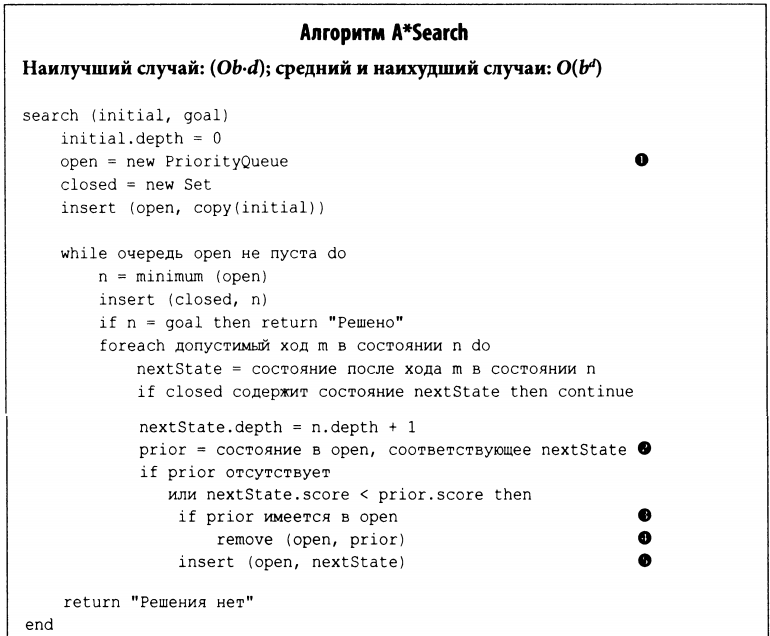
\includegraphics[scale=0.5]{images/lec06-pic08.png}
\end{figure}
\end{frame}

\begin{frame}
\begin{figure}[h]
\centering

\includegraphics[scale=0.6]{images/lec06-pic09.png}
\end{figure}
\end{frame}

\begin{frame}{Входные и выходные параметры алгоритма A*Search}
\begin{itemize}
\item Алгоритм начинает работу с начального состояния доски в дереве поиска и целевого состояния. 
\item Он предполагает наличие функции оценки $f(n)$ с приемлемой функцией $h(n)$.
\item Алгоритм возвращает последовательность ходов, являющуюся решением,
которое наиболее близко приближается к решению с минимальной стоимостью, переводящему первоначальное состояние в целевое (или объявляет, что такое решение не может быть найдено при имеющихся в наличии ресурсах).
\end{itemize}
\end{frame}

\begin{frame}{Пример работы алгоритма}
Начальное состояние доски для алгоритма А *Search:
\begin{figure}[h]
\centering
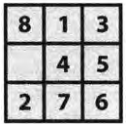
\includegraphics[scale=0.6]{images/lec06-pic10.png}
\end{figure}
\begin{itemize}
\item Для примера головоломки <<8>> с начальным состоянием, показанным на рисунке.
\item Дерево на следующем слайде использует функцию $f(n)$ \textit{GoodEvaluator}, предложенную в \textit{Nilsson, N., Problem-Solving Methods in Artificial Intelligence. McGraw-Hill, 1971}. 
\item Через слайд использована функция \textit{WeakEvaluator} из той же работы. 
\item Светло-серый цвет состояния показывает множество открытых состояний в момент достижения целевого состояния.
\end{itemize}
\end{frame}

\begin{frame}
Пример дерева A*Search при использовании функции GoodEvaluator
\begin{figure}[h]
\centering
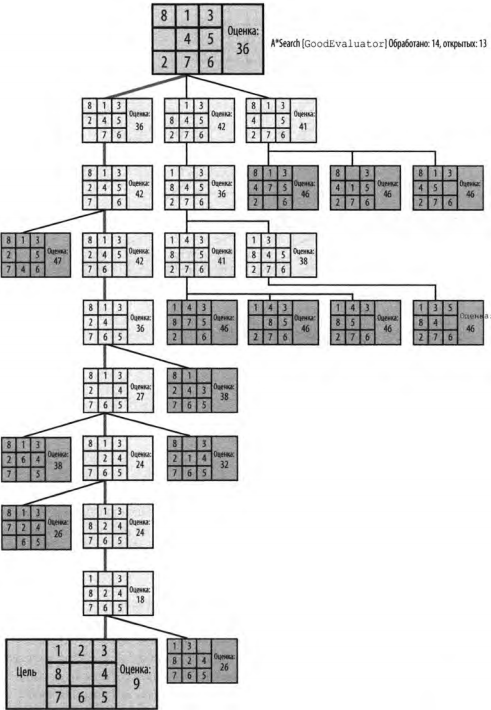
\includegraphics[scale=0.4]{images/lec06-pic11.png}
\end{figure}
\end{frame}

\begin{frame}
Пример дерева A*Search при использовании функции WeakEvaluator
\begin{figure}[h]
\centering
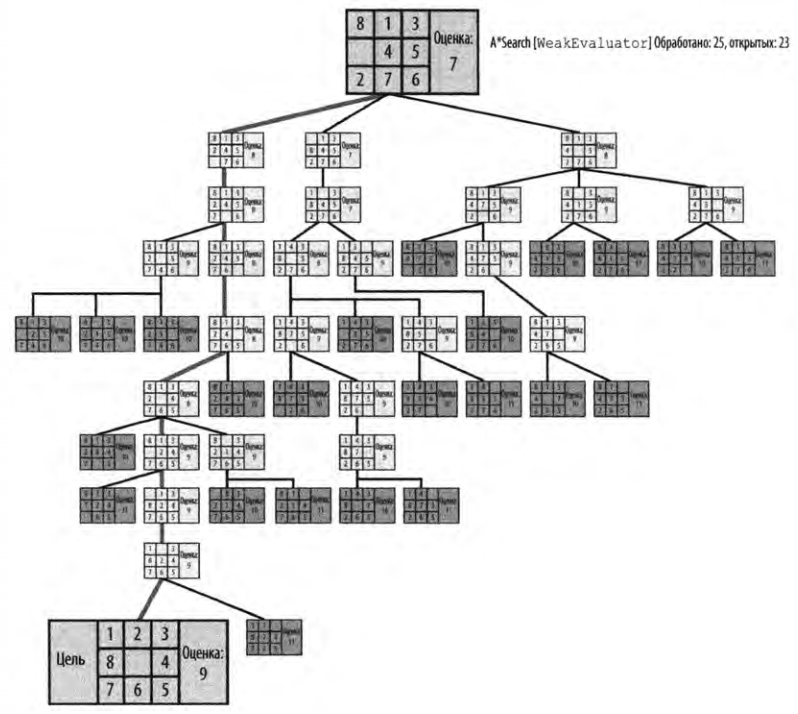
\includegraphics[scale=0.4]{images/lec06-pic12.png}
\end{figure}
\end{frame}

\begin{frame}
\begin{itemize}
\item Обе функции находят одно и то же решение из девяти ходов в целевой узел, но поиск с использованием функции GoodEvaluator оказывается более эффективным. 
\item Заметим, что через два хода от первоначального состояния в дереве поиска GoodEvaluator начинается четкий путь из узлов с постоянно уменьшающимся значением $f(n)$, который приводит к целевому узлу. 
\item В дереве же поиска WeakEvaluator приходится исследовать четыре хода от исходного состояния до того, как направление поиска будет сужено.
\item WeakEvaluator неверно различает состояния доски; значение $f(n)$ целевого узла оказывается выше, чем значения f(n) для начального узла и всех трех его дочерних узлов.
\end{itemize}
\end{frame}

\begin{frame}
\begin{itemize}
\item Успех алгоритма A*Search непосредственно зависит от его эвристической функции. 
\item Компонент $h(n)$ функции оценки $f(n)$ должен быть тщательно разработан, и это в большей степени искусство, чем наука. 
\item Если h(n) всегда равно нулю, A*Search вырождается в простой поиск в ширину. 
\item Кроме того, если $h(n)$ переоценивает стоимость достижения целевого состояния, A*Search может не суметь найти оптимальное решение, хотя и сможет возвратить какое-то решение в предположении, что $h(n)$
не слишком далека от истины. 
\item A*Search будет находить оптимальное решение, если эвристическая функция $h(n)$ является приемлемой.
\end{itemize}
\end{frame}

\begin{frame}
\begin{itemize}
\item Большая часть литературы, посвященной A*Search, описывает высокоспециализированные функции $h(n)$ для разных областей, таких как поиск маршрута на цифровой местности [1] или планирование проектов при ограниченных ресурсах [2]. 
\item Книга [3] представляет собой обширный справочник по разработке эффективных эвристик. 
\item В [4] описывается, как создавать приемлемые функции $h(n)$, а в [5] приведены последние перспективы использования эвристик в решении задач, и не только для A*Search.
\end{itemize}
\end{frame}

\begin{frame}
\begin{enumerate}
\item Wichmann, D. and B. Wuensche, <<Automated route finding on digital terrains>>, Proceedings of IVCNZ, Akaroa, New Zealand, pp. 107-112, November 2004, https://www.researchgate.net/publication/
245571114\_Automated\_Route\_Finding\_on\_Digital\_Terrains.
\item Hartmann, S., Project Scheduling Under Limited Resources: Models, Methods, and Applications. Springer, 1999.
\item Pearl, J., Heuristics: Intelligent Search Strategies for Computer Problem Solving. AddisonWesley, 1984
\item Korf, R. Е., <<Recent progress in the design and analysis of admissible heuristic functions>>, Proceedings, Abstraction, Reformulation, and Approximation: 4th International Symposium (SARA), Lecture notes in Computer Science \#1864: 45-51, 2000, http://www.aaai.org/Papers/AAAI/2000/AAAI00-212.pdf.
\item Michalewicz, Z. and D. Fogel, How to Solve It: Modern Heuristics. Second Edition. Springer, 2004.
\end{enumerate}
\end{frame}

\begin{frame}{Функции h(n) для головоломки <<>8>}
\begin{itemize}
\item FairEvaluator ::= $Р(n)$, где $Р(n)$ - это сумма манхэттенских расстояний каждой плитки от ее окончательного местоположения.
\item GoodEvaluator ::= $P(h)+3-S(h)$, где $Р(n)$ определена выше, a $S(n)$ представляет собой оценку последовательности, которая по очереди проверяет нецентральные квадраты, давая $0$ для каждой плитки, за которой идет ее корректный преемник, и $2$ для плитки, не обладающей этим свойством; плитка в центре получает оценку $1$.
\item WeakEvaluator - Подсчет количества плиток, находящихся не на своем месте.
\item BadEvaluator - Общая разность противоположных (относительно центра) плиток по сравнению с идеальным значением, равным 16.
\end{itemize}
\end{frame}

\begin{frame}
Пример состояния доски для тестирования функций оценки
\begin{figure}[h]
\centering
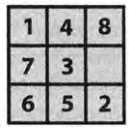
\includegraphics[scale=0.5]{images/lec06-pic13.png}
\end{figure}
Сравнение трех приемлемых и одной неприемлемой функций h(n):
\begin{figure}[h]
\centering
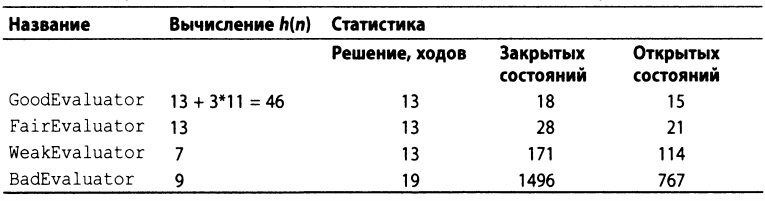
\includegraphics[scale=0.6]{images/lec06-pic14.png}
\end{figure}
\end{frame}

\begin{frame}
\begin{itemize}
\item Чем более сложными становятся состояния доски, тем большую важность приобретают эвристические функции и тем более сложной становится их разработка. 
\item Они должны оставаться эффективно вычисляемыми, иначе процесс поиска резко замедлится.
\end{itemize}
\begin{figure}[h]
\centering
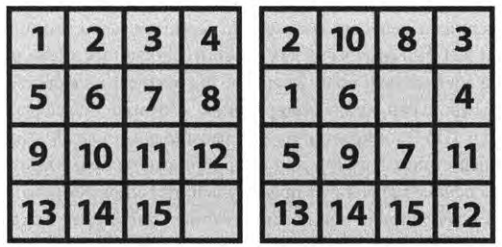
\includegraphics[scale=0.4]{images/lec06-pic15.png}
\end{figure}
\begin{itemize}
\item Для целевого состояния (слева) и начального состояния (справа) A*Search GoodEvaluator быстро находит решение из 15 ходов после обработки 39 состояний доски. 
\item По окончании работы во множестве открытых состояний остаются 43 непросмотренных состояния.
\end{itemize}
\end{frame}

\begin{frame}
При попытке решения для более сложного начального состояния алгоритм A*Search исчерпывает всю доступную память.
\begin{figure}[h]
\centering
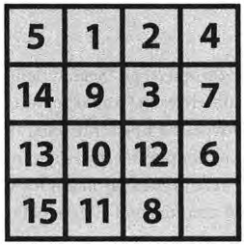
\includegraphics[scale=0.4]{images/lec06-pic16.png}
\end{figure}
\end{frame}

\begin{frame}
В таблице содержатся итоговые результаты 1000 испытаний, где $n$ — количество случайных ходов (от 2 до 14): 
\begin{itemize}
\item данные о среднем количестве состояний в сгенерированных деревьях поиска 
\item среднее количество ходов в найденных решениях. 
\item BFS означает поиск в ширину, DFS - поиск в глубину и А - поиск A*Search.
\end{itemize}
\begin{figure}[h]
\centering
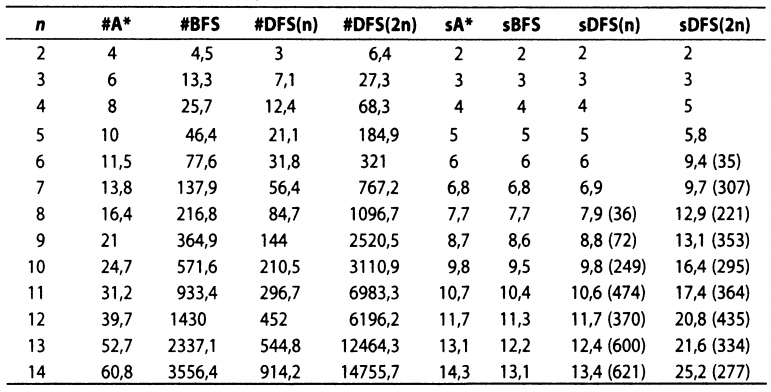
\includegraphics[scale=0.5]{images/lec06-pic17.png}
\end{figure}
\end{frame}

\begin{frame}
Темпы роста для слепых поисков приближены следующими функциями: 

\[BFS(n) \cong 0,24\dot (n+1)^{2.949}\]
\[DFS(n) \cong 1,43\dot (n+1)^{2,275}\]
\[DFS(2n) \cong 3,18\dot (n+1)^{3,164}\].

В отдельных испытаниях для A*Search с 30 случайными ходами темп роста дерева поиска был оценен как $0(n^{1.5147})$, хотя этот рост и не линейный, размер дерева оказывается значительно меньше, чем для слепых поисков.
\end{frame}

\begin{frame}{Сравнение размеров деревьев поиска для случайных позиций}
\begin{figure}[h]
\centering
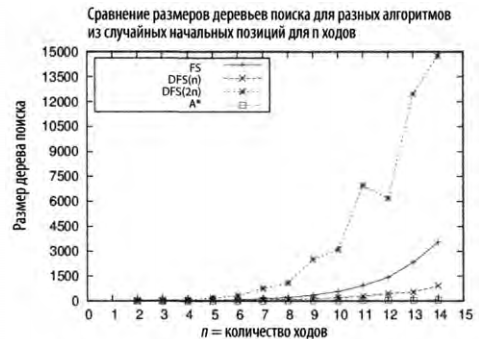
\includegraphics[scale=0.75]{images/lec06-pic18.png}
\end{figure}
\end{frame}

\begin{frame}{Сравнение размеров деревьев поиска для случайных позиций}
\begin{figure}[h]
\centering
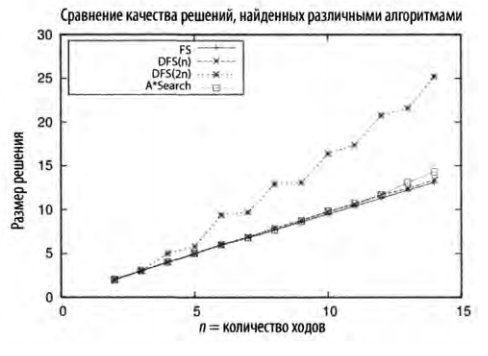
\includegraphics[scale=0.75]{images/lec06-pic19.png}
\end{figure}
\end{frame}

\end{document}